% Created 2012-11-02 Fri 20:19
\documentclass[11pt]{article}
\usepackage[latin1]{inputenc}
\usepackage{fixltx2e}
\usepackage{url}
\usepackage{graphicx}
\usepackage{minted}
\usepackage{color}
\usepackage{longtable}
\usepackage{float}
\usepackage{wrapfig}
\usepackage{soul}
\usepackage{textcomp}
\usepackage{amsmath}
\usepackage{marvosym}
\usepackage{wasysym}
\usepackage{latexsym}
\usepackage{amssymb}
\usepackage[linktocpage,
  pdfstartview=FitH,
  colorlinks,
  linkcolor=blue,
  anchorcolor=blue,
  citecolor=blue,
  filecolor=blue,
  menucolor=blue,
  urlcolor=blue]{hyperref}
\usepackage{attachfile}
\tolerance=1000
\providecommand{\alert}[1]{\textbf{#1}}

\title{readme}
\author{}
\date{\today}
\hypersetup{
  pdfkeywords={},
  pdfsubject={},
  pdfcreator={Emacs Org-mode version N/A-fixup}}

\begin{document}

\maketitle

\setcounter{tocdepth}{3}
\tableofcontents
\vspace*{1cm}
\section{Mini Project 1}
\label{sec-1}
\subsection{Problem}
\label{sec-1-1}

There are many ways to visualize the electron density.  One way is to plot it as a ``fog'' or cloud-like where the colormap represents the charge density of the electron cloud in a compound.
\subsection{Method}
\label{sec-1-2}

The ``fog'' is plotted using in-built functions of mayavi, jasp, and some short scripts written to grab data from the OUTCAR and CHG files produced by VASP.  In the attached plots, the deeper the red color, the higher is the charge density.
\subsection{Files}
\label{sec-1-3}

Two scripts are written:


\begin{enumerate}
\item mini\_v2.org
\end{enumerate}


This includes the jasp commands to retrieve the VASP outputs, function calls to retrieve additional data, and the actual plotting.


The structure of this file:


a. Inputs.


b. Use of jasp to retrieve data from VASP output files.


c. Read CHG to get position of the atoms and plot them.


d. Read OUTCAR to get linkages and plot them if needed.


e. Plot simulation cell boundary if needed.


f. Plot the electron charge density.


g. Save the figure. (Default: Isometric view but other relevant views can be saved)
\subsection{How to use}
\label{sec-1-4}

Steps to use this code:


a. Copy the 2 files listed above (mini\_v2.org and getPosLink.py) into a new folder created in a machine that has jasp.


b. Copy the output folder containing the output files from VASP calculation into this new folder


c. In the mini\_v2.org,


      i.   Put in the name of this output folder in variable calDir (e.g., calDir = `h2o').

      ii.  Indicate if u want to plot the linkage between atoms and the simulation cell boundary.

      iii. It is ready to go.

(attached in the folder is a sample output folder from VASP for h2o molecule)
\subsubsection{Example of input needed (reproduced from mini\_v2.org)}
\label{sec-1-4-1}


\#\#\#\# Inputs required from user from HERE \#\#\#\#\#\#

dirCal = `h2o'

\#1 to plot linkage between atoms (for simple molecules), 0 otherwise

plotLinks = 1


\#1 to plot cell boundary, 0 otherwise

plotCell= 0

\#\#\#\#\#\#\#\#\#    To HERE   \#\#\#\#\#\#\#\#\#\#\#\#\#\#\#\#\#\#\#
\subsection{Limitations}
\label{sec-1-5}

No known limitation for the plotting of electron density except the need for jasp and other softwares/libraries imported in mini\_v2.org and getPosLink.py.  Simple molecules, periodic crystal structures, non-symmetrical and non-cubic lattices, and unit cell with a molecule that was not centered were tested.


The only limitation comes from the plotting of linkages between atoms.  This is done based on the nearest neighbour list in OUTCAR.  It does not know and cannot plot the presence of multiple bonds between atom pairs (e.g., double or triple bond in C2H4 and C2H2)


The color of each atom is arbitrary.  Atoms are of the same size in the  plots below but can be scaled arbitrary.
\subsection{Images of electron density for several materials}
\label{sec-1-6}


The single molecule images are generated using ENCUT = 300 except otherwise stated.  The periodic structures are generated with converged ENCUT and K-PTS.
\subsubsection{Single molecules}
\label{sec-1-6-1}
\begin{itemize}

\item H2O\\
\label{sec-1-6-1-1}%
Top view
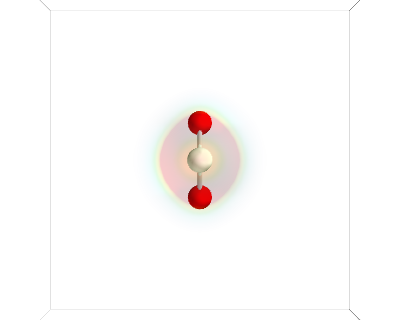
\includegraphics[width=.9\linewidth]{./images/h2o_top.png}

Iso view
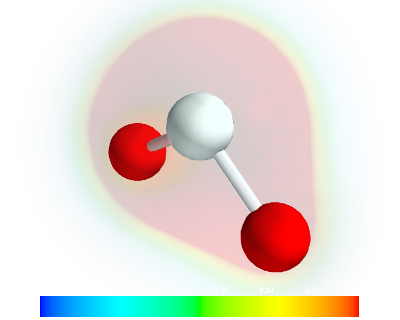
\includegraphics[width=.9\linewidth]{./images/h2o_iso.png}

Side view
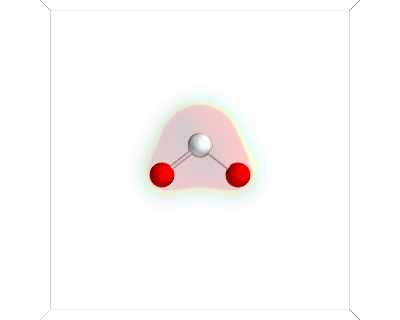
\includegraphics[width=.9\linewidth]{./images/h2o_side.png}

Front view
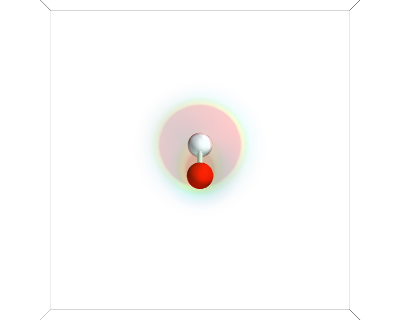
\includegraphics[width=.9\linewidth]{./images/h2o_front.png}


\item H2O (with different ENCUT)\\
\label{sec-1-6-1-2}%
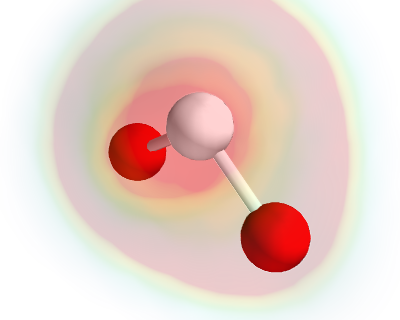
\includegraphics[width=.9\linewidth]{./images/h2o-100_iso.png}

ENCUT = 100

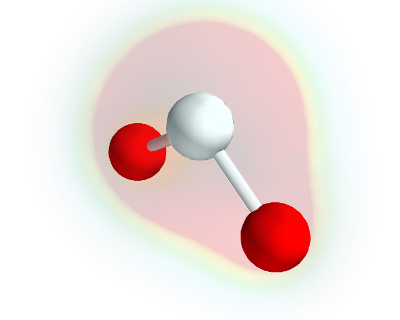
\includegraphics[width=.9\linewidth]{./images/h2o-400_iso.png}

ENCUT = 400

There is a difference in the electron density.  The difference itself is not shown in a single plot as the electron density grid for ENCUT = 400 is more finely divided than ENCUT = 100.  This creates a need to interpolate between the points for ENCUT = 100 to get an equal sized matrix.  From these two plots, the electron density spans a larger area at smaller ENCUT and has a higher density at a certain region around the molecule.


\item CH3COF (4 elements)\\
\label{sec-1-6-1-3}%
Top view
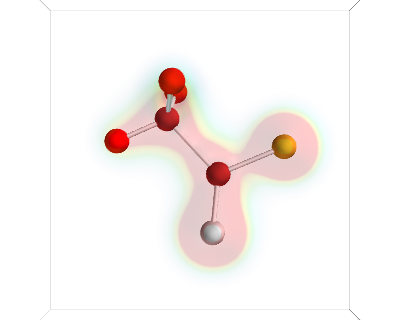
\includegraphics[width=.9\linewidth]{./images/CH3COF_top.png}

Iso view
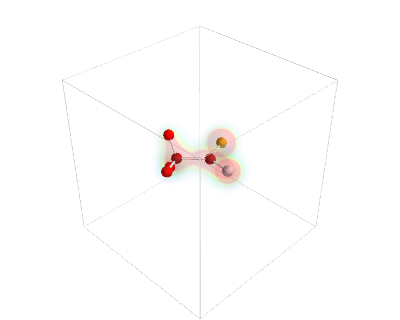
\includegraphics[width=.9\linewidth]{./images/CH3COF_iso.png}

Side view
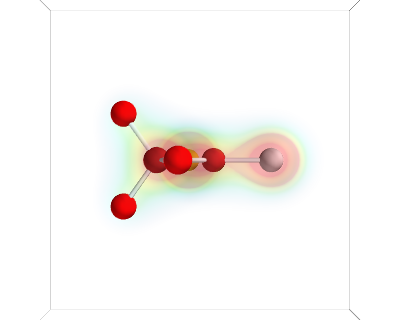
\includegraphics[width=.9\linewidth]{./images/CH3COF_side.png}

Front view
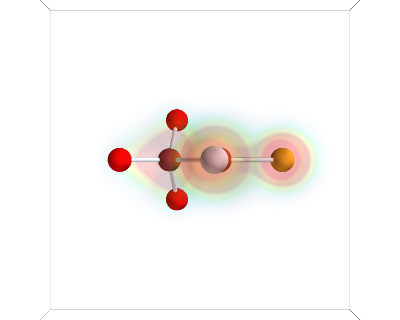
\includegraphics[width=.9\linewidth]{./images/CH3COF_front.png}

There is a localisation of the electron density around the F and O atoms (yellow and white spheres) as they are more electronegtive.


\item NH3 (Lone pair of electrons)\\
\label{sec-1-6-1-4}%
Top view
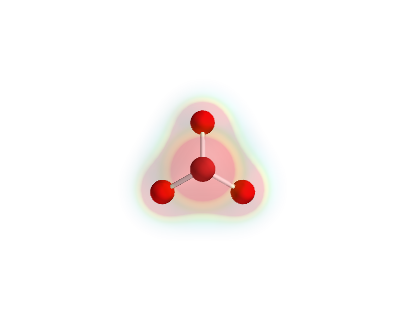
\includegraphics[width=.9\linewidth]{./images/NH3_top.png}

Iso view
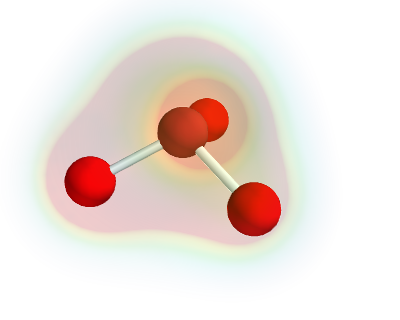
\includegraphics[width=.9\linewidth]{./images/NH3_iso.png}

Side view
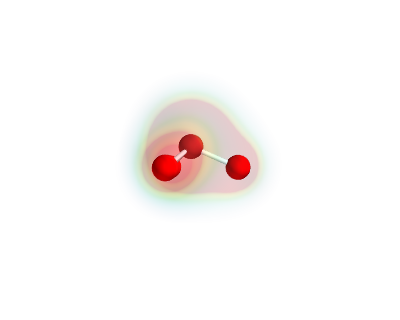
\includegraphics[width=.9\linewidth]{./images/NH3_side.png}

Front view
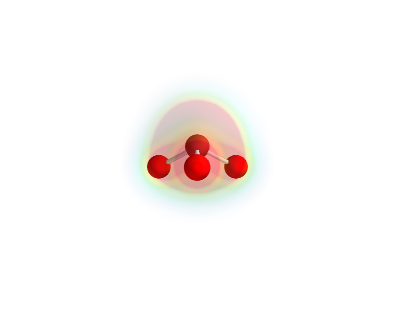
\includegraphics[width=.9\linewidth]{./images/NH3_front.png}

From the front view, there is a bulge in the electron density above the central N-atom (dark red) that has a lone pair of electrons.


\item C6H6 (Benzene)\\
\label{sec-1-6-1-5}%
Top view
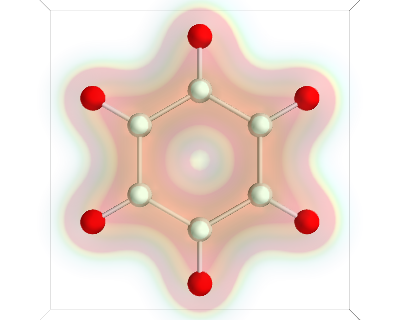
\includegraphics[width=.9\linewidth]{./images/C6H6_top.png}

Iso view
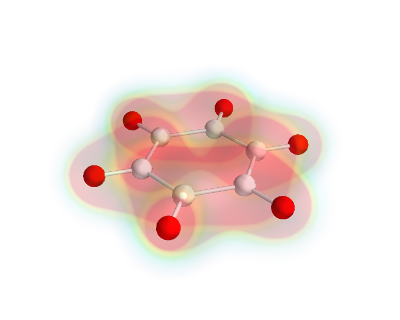
\includegraphics[width=.9\linewidth]{./images/C6H6_iso.png}

Side view
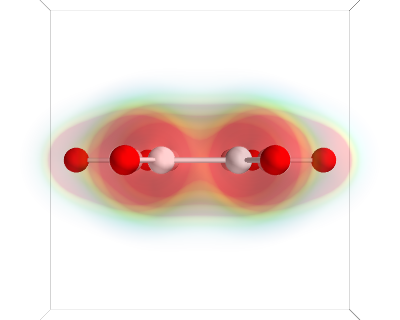
\includegraphics[width=.9\linewidth]{./images/C6H6_side.png}

Front view
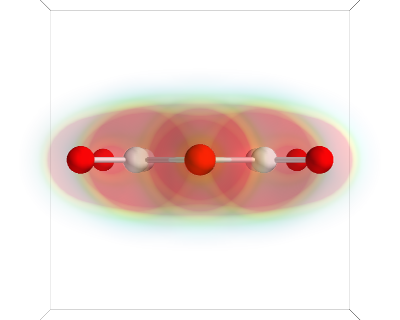
\includegraphics[width=.9\linewidth]{./images/C6H6_front.png}

There is a concentration of electron density along the carbon backbone forming a ring. A lack of electron density in the center is observed.  This mirrors the bonding nature in benzene.


\item C2H2 (Triple Bond in carbon chain)\\
\label{sec-1-6-1-6}%
Top view
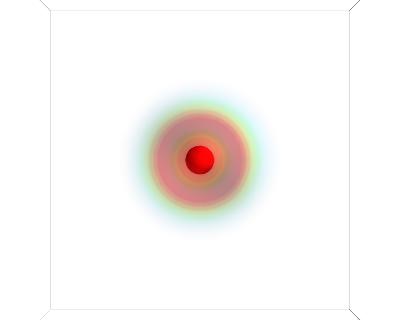
\includegraphics[width=.9\linewidth]{./images/C2H2_top.png}

Iso view
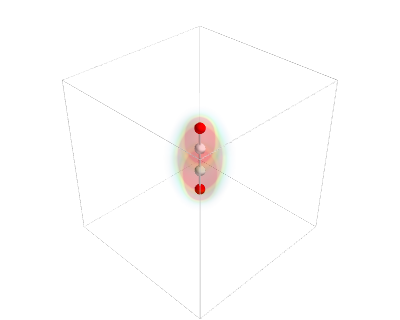
\includegraphics[width=.9\linewidth]{./images/C2H2_iso.png}

Side view
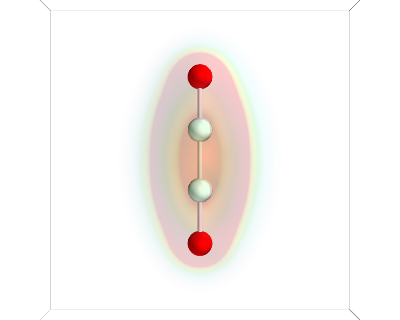
\includegraphics[width=.9\linewidth]{./images/C2H2_side.png}

Front view
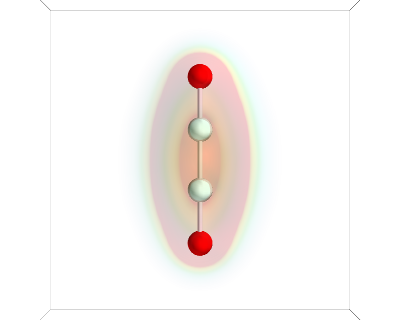
\includegraphics[width=.9\linewidth]{./images/C2H2_front.png}


\item C2H4 (Double Bond in carbon chain)\\
\label{sec-1-6-1-7}%
Top view
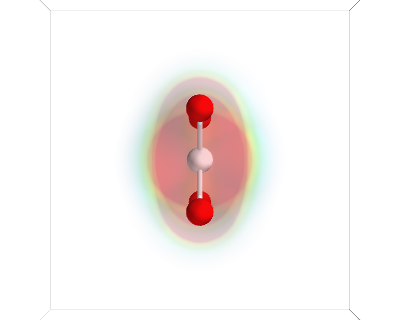
\includegraphics[width=.9\linewidth]{./images/C2H4_top.png}

Iso view
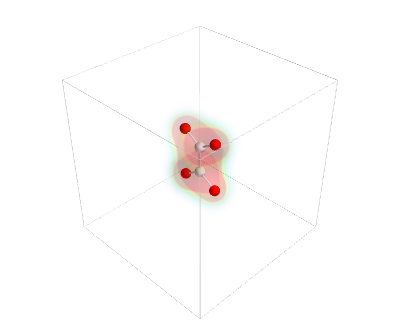
\includegraphics[width=.9\linewidth]{./images/C2H4_iso.png}

Side view
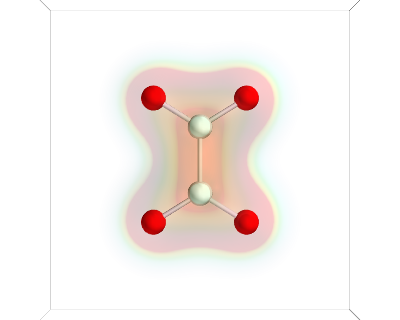
\includegraphics[width=.9\linewidth]{./images/C2H4_side.png}

Front view
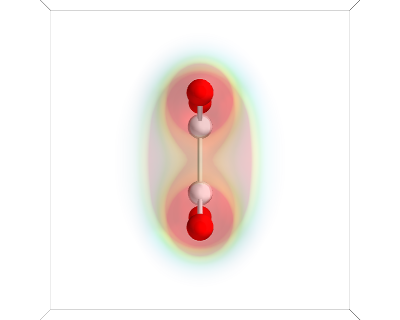
\includegraphics[width=.9\linewidth]{./images/C2H4_front.png}


\item C2H6 (Single Bond in carbon chain)\\
\label{sec-1-6-1-8}%
Top view
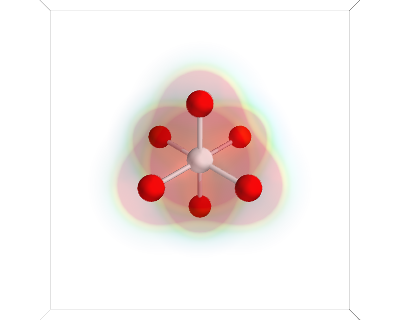
\includegraphics[width=.9\linewidth]{./images/C2H6_top.png}

Iso view
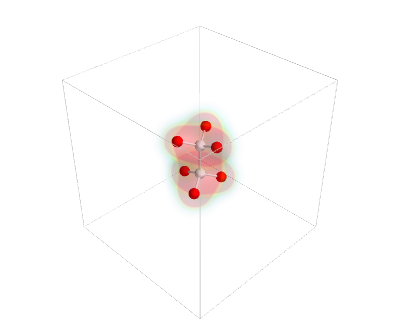
\includegraphics[width=.9\linewidth]{./images/C2H6_iso.png}

Side view
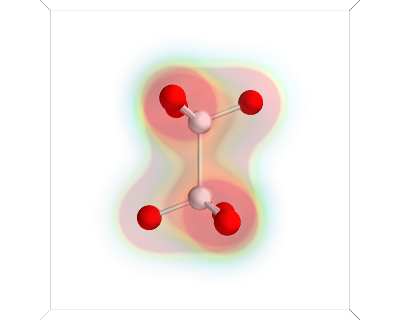
\includegraphics[width=.9\linewidth]{./images/C2H6_side.png}

Front view
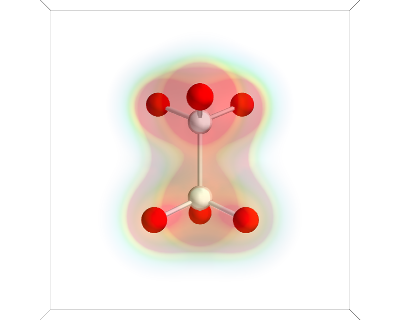
\includegraphics[width=.9\linewidth]{./images/C2H6_front.png}

Comparison between images of C2H2, C2H4 and C2H6 shows a higher electron density between the carbon pair for C2H2 and C2H4 than for C2H6.  This is due to the presence of the double and triple bond.


\item C2H6 (Not Centered)\\
\label{sec-1-6-1-9}%
Top view
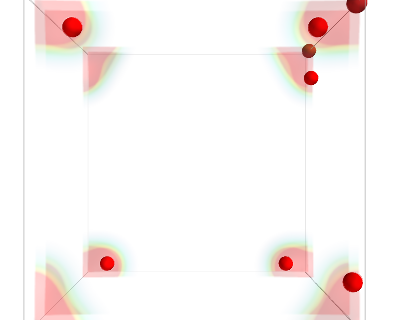
\includegraphics[width=.9\linewidth]{./images/C2H6-notCenter_top.png}

Iso view
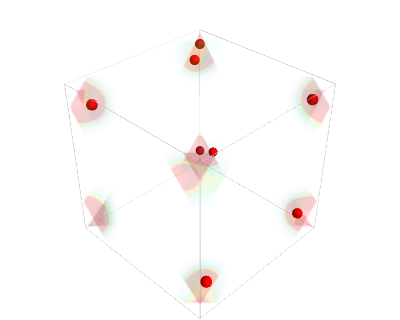
\includegraphics[width=.9\linewidth]{./images/C2H6-notCenter_iso.png}

Side view
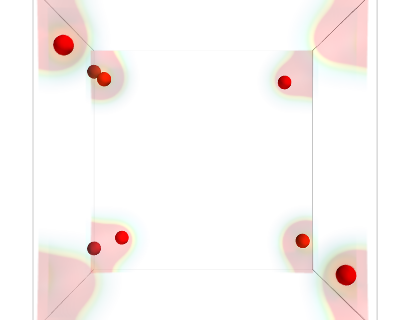
\includegraphics[width=.9\linewidth]{./images/C2H6-notCenter_side.png}

Front view
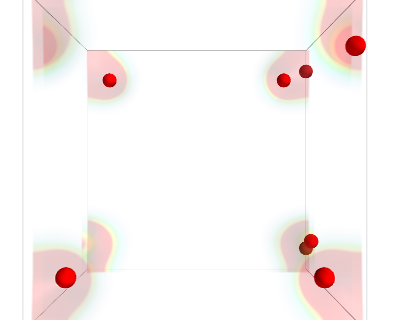
\includegraphics[width=.9\linewidth]{./images/C2H6-notCenter_front.png}


\item CO2\\
\label{sec-1-6-1-10}%
Top view
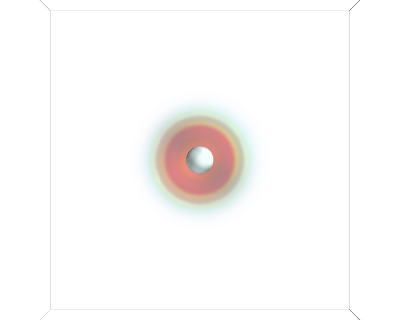
\includegraphics[width=.9\linewidth]{./images/co2_top.png}

Iso view
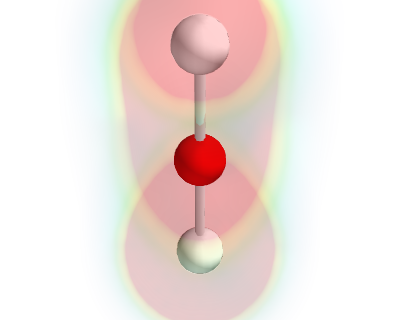
\includegraphics[width=.9\linewidth]{./images/co2_iso.png}

Side view
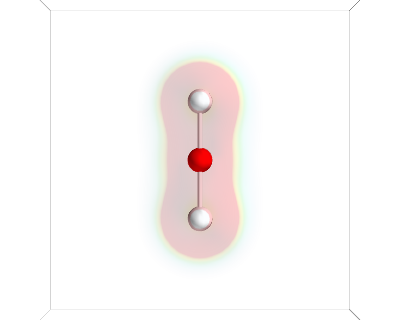
\includegraphics[width=.9\linewidth]{./images/co2_side.png}

Front view
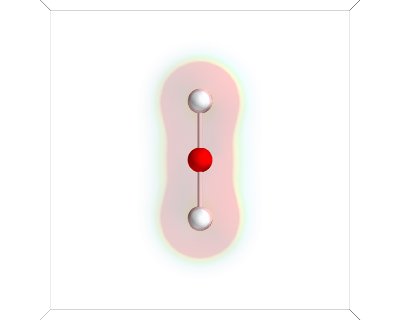
\includegraphics[width=.9\linewidth]{./images/co2_front.png}



\item CO2 (Non-uniform simulation cubic cell)\\
\label{sec-1-6-1-11}%
Top view
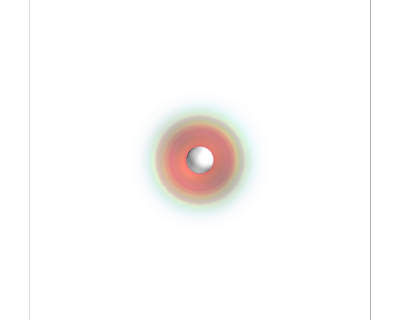
\includegraphics[width=.9\linewidth]{./images/co2-diffsize_top.png}

Iso view
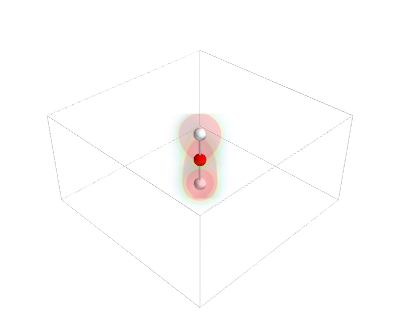
\includegraphics[width=.9\linewidth]{./images/co2-diffsize_iso.png}

Side view
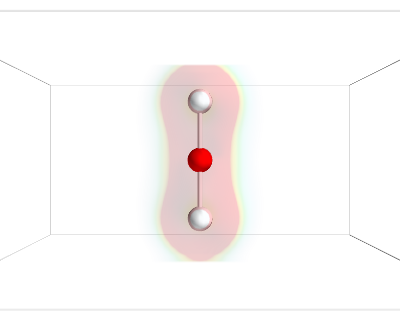
\includegraphics[width=.9\linewidth]{./images/co2-diffsize_side.png}

Front view
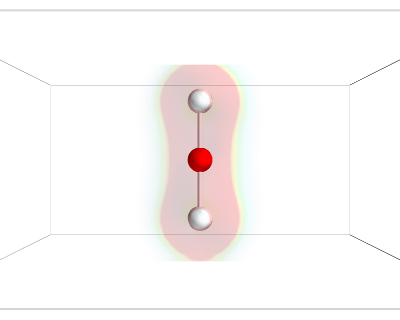
\includegraphics[width=.9\linewidth]{./images/co2-diffsize_front.png}



\end{itemize} % ends low level
\subsubsection{Periodic structures}
\label{sec-1-6-2}


These periodicity of these cells result in plots of electron density not being self-contained but spreads across the cell boundary.
\begin{itemize}

\item Ta (BCC Metal)\\
\label{sec-1-6-2-1}%
Top view
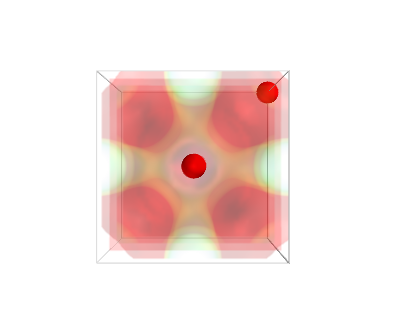
\includegraphics[width=.9\linewidth]{./images/Ta_top.png}

Iso view
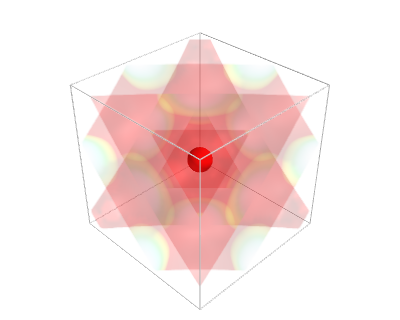
\includegraphics[width=.9\linewidth]{./images/Ta_iso.png}

Side view
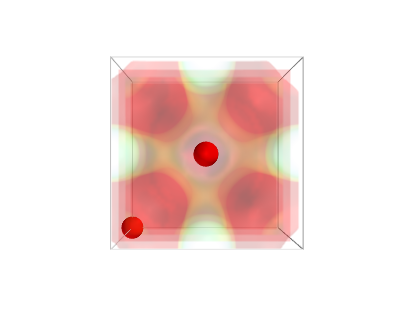
\includegraphics[width=.9\linewidth]{./images/Ta_side.png}

Front view
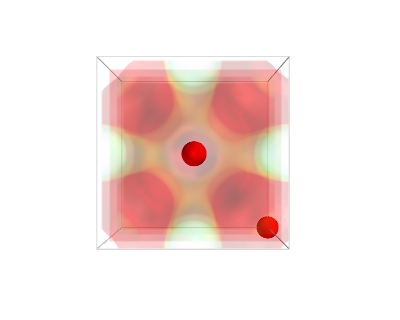
\includegraphics[width=.9\linewidth]{./images/Ta_front.png}

The electron cloud tends to cluster near to the center and vertices of the cell in constrast to the rock-salt structure of TaC shown below.


\item Graphite (Planar hexagonal)\\
\label{sec-1-6-2-2}%
Top view
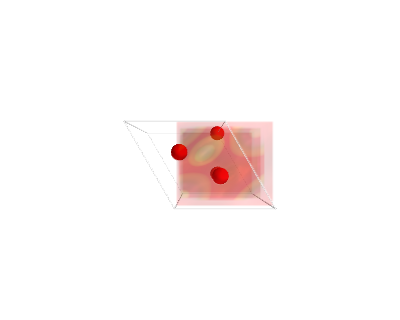
\includegraphics[width=.9\linewidth]{./images/cGraph_top.png}

Iso view
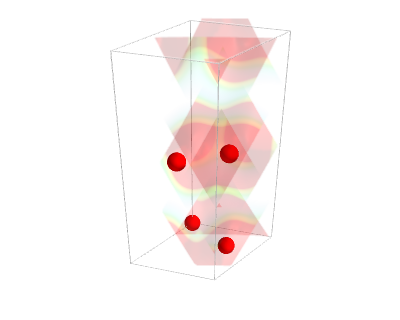
\includegraphics[width=.9\linewidth]{./images/cGraph_iso.png}

Side view
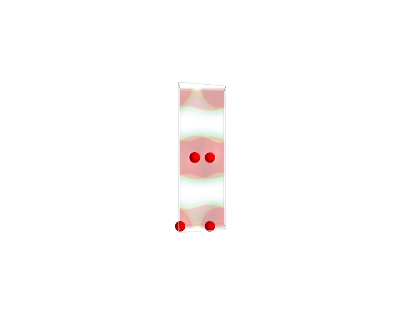
\includegraphics[width=.9\linewidth]{./images/cGraph_side.png}

Front view
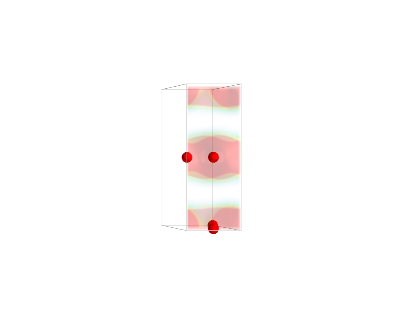
\includegraphics[width=.9\linewidth]{./images/cGraph_front.png}

The electron density is separated into distinct layers, similar to the physical atomic arrangement in graphite.


\item TaC (rock-salt structure)\\
\label{sec-1-6-2-3}%
Top view
\includegraphics[width=.9\linewidth]{./images/TaC_top.png}

Iso view
\includegraphics[width=.9\linewidth]{./images/TaC_iso.png}

Side view
\includegraphics[width=.9\linewidth]{./images/TaC_side.png}

Front view
\includegraphics[width=.9\linewidth]{./images/TaC_front.png}

There are more ``hollow'' regions enclosed within the simulation cell in this rock-salt structure  as compared to the BCC Ta.  The number density and arrangement of the atoms in this structure differ from BCC, pulling electrons closer around each atom.
\end{itemize} % ends low level

\end{document}
